% Topic control -- appendix material for Report 2 (final corrected version, 2026-10-29).
% \input this in the same document as topic_control_section.tex (e.g. after the main
% sections, before the bibliography), so the cross-references resolve.

\subsection*{Appendix: Topic Control Supplementary Results}

\begin{table}[H]
\centering
\caption{Pooled automated lexical follow-up rate when a fixed TF-IDF similarity threshold is used instead of the episode median (131 mixed-gender episodes, 17,046 initiations). Gaps are male $-$ female; 95\% CIs from 500 episode-level bootstrap samples. Not adjusted for role: 78\% of male and 30\% of female initiations come from hosts.}
\label{tab:tc-thresholds}
\begin{tabular}{cccc}
\toprule
Threshold & Female & Male & Male $-$ female (pp) [95\% CI] \\
\midrule
0.02 & 33.4\% & 37.8\% & 4.4 [1.9, 7.0] \\
0.05 & 21.7\% & 25.3\% & 3.5 [1.1, 5.9] \\
0.10 & 11.9\% & 15.2\% & 3.4 [1.6, 4.9] \\
0.15 &  7.6\% & 10.2\% & 2.6 [1.3, 3.8] \\
0.20 &  5.1\% &  7.5\% & 2.4 [1.4, 3.3] \\
0.30 &  2.9\% &  4.1\% & 1.3 [0.5, 1.9] \\
\bottomrule
\end{tabular}
\end{table}

\begin{table}[H]
\centering
\caption{Paired within-episode comparison of the male and female speaker in the 131 mixed-gender episodes, with TF-IDF and sentence-embedding (all-MiniLM-L6-v2) similarity. Values are means of episode-level follow-up rates; gap = male $-$ female with $t$-based 95\% CI; paired $t$-test and 10,000 sign-flip permutations. Not adjusted for role. The embedding measure selects its own initiations (15,799 vs.\ 17,046).}
\label{tab:tc-within}
\small
\begin{tabular}{lcccccc}
\toprule
Similarity & Initiations & Female & Male & Gap (pp) [95\% CI] & Paired $t$ ($p$) & Permutation $p$ \\
\midrule
TF-IDF     & 17,046 & 42.6\% & 41.5\% & $-1.2$ [$-4.1$, $+1.8$] & $-0.78$ (0.44) & 0.44 \\
Embeddings & 15,799 & 48.4\% & 47.2\% & $-1.2$ [$-4.1$, $+1.8$] & $-0.78$ (0.43) & 0.44 \\
\bottomrule
\end{tabular}
\end{table}

\begin{figure}[H]
\centering
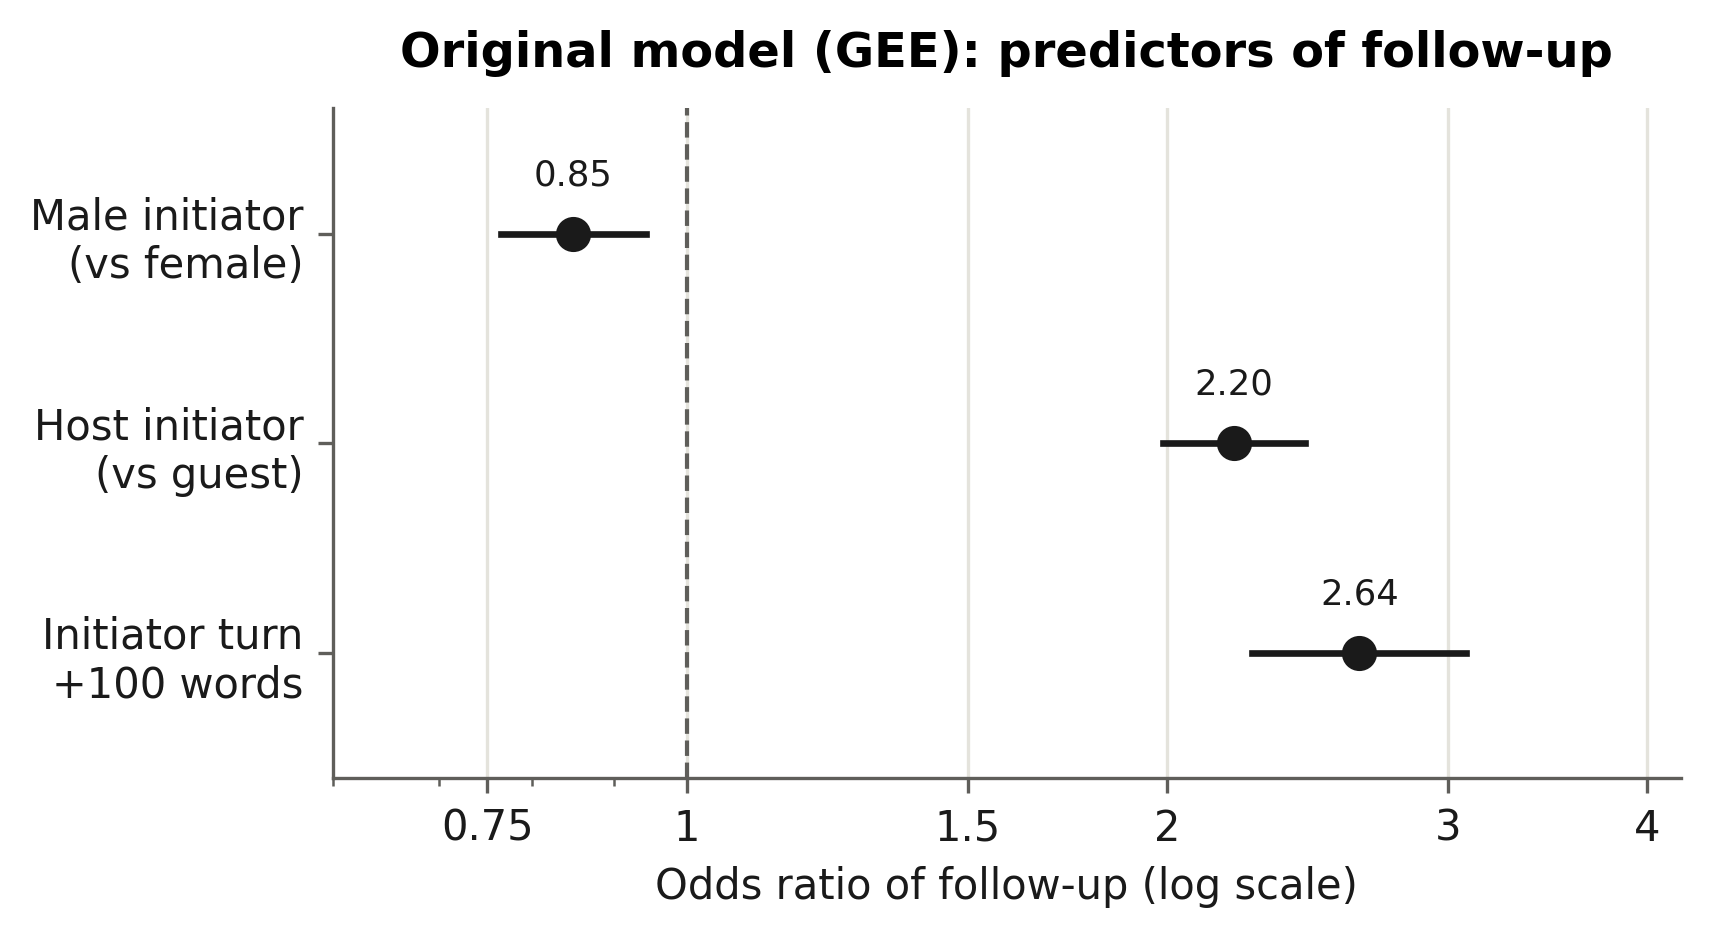
\includegraphics[width=0.6\linewidth]{figures/fig4_gee_original_model.png}
\caption{Odds ratios (95\% CI, log scale) from the original GEE model of binary automated lexical follow-up (131 mixed-gender episodes, 17,046 initiations; robust errors grouped by episode). Turn length is per 100 words of the initiating turn. The gender estimate is not robust to how turn length is modelled (Table~\ref{tab:tc-sensitivity}).}
\label{fig:tc-gee}
\end{figure}

\begin{figure}[H]
\centering
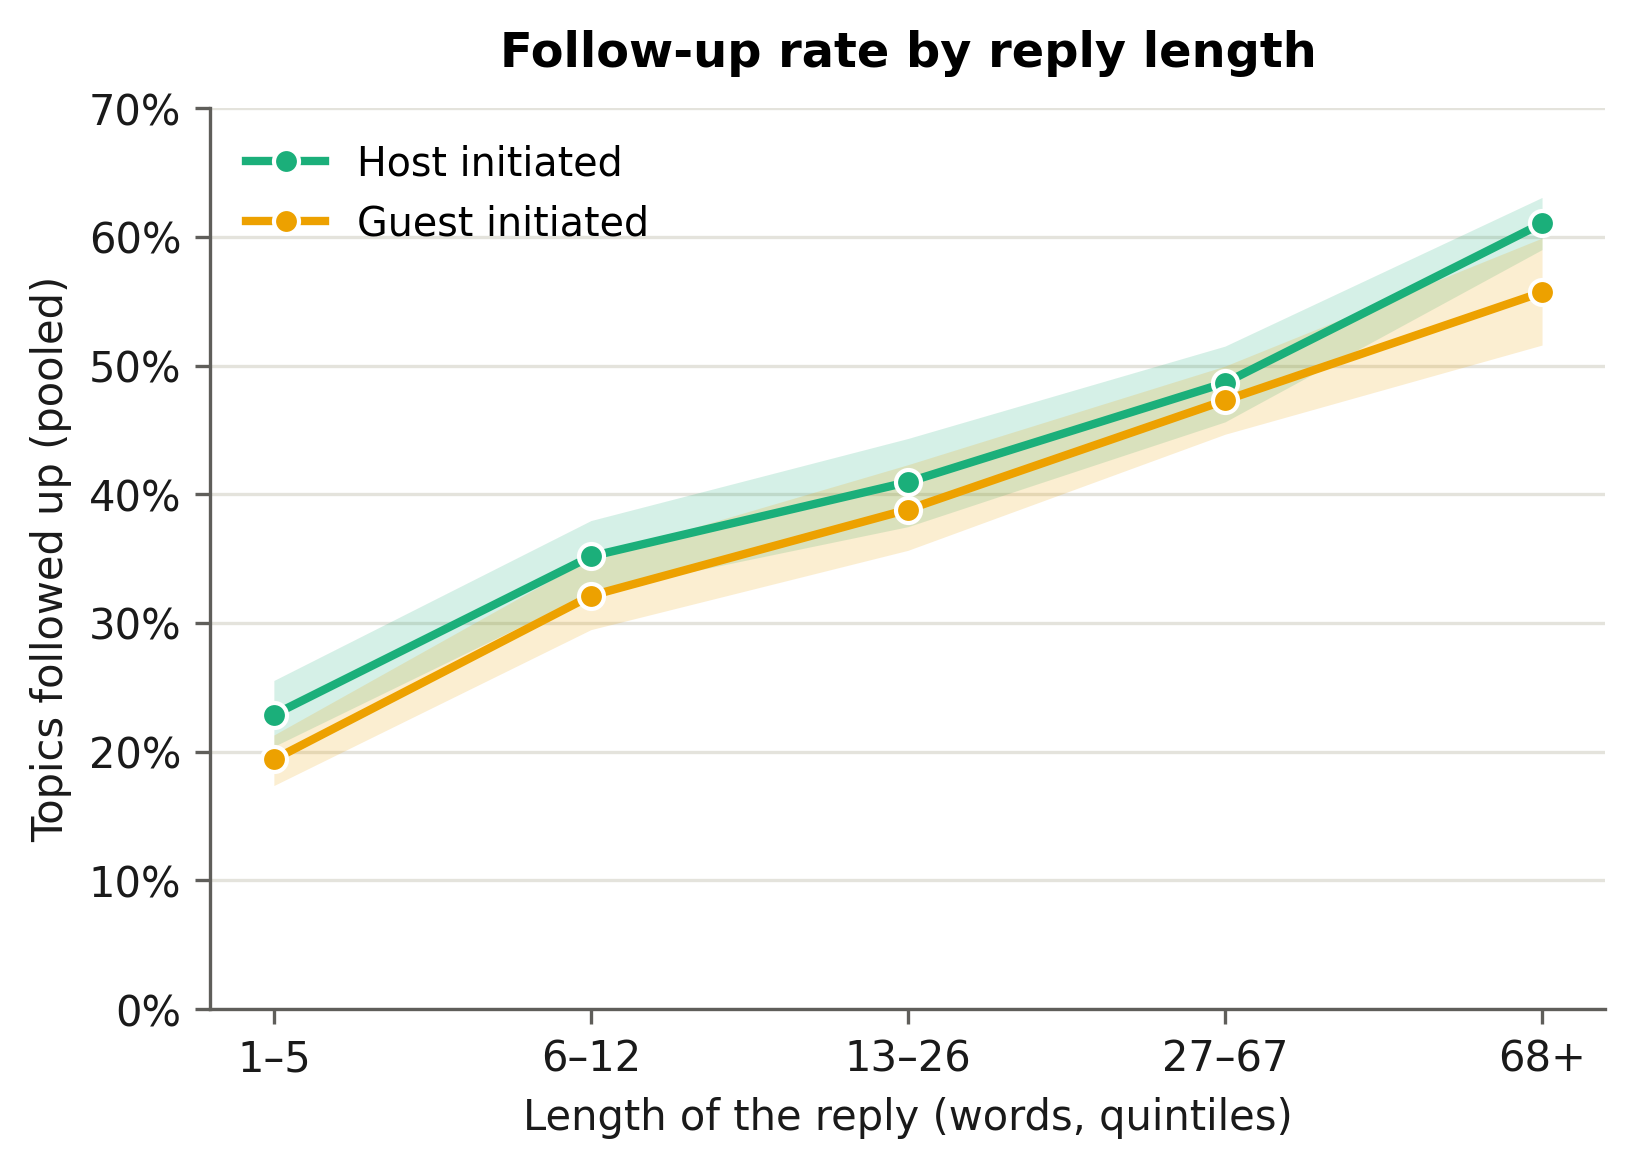
\includegraphics[width=0.6\linewidth]{figures/fig6_followup_by_reply_length.png}
\caption{Pooled automated lexical follow-up rate by reply length (quintiles of reply word count) for host- and guest-initiated topics (131 mixed-gender episodes). Bands are 95\% CIs from 1,000 episode-level bootstrap samples. Longer replies are more likely to share a content word with the initiating turn.}
\label{fig:tc-length}
\end{figure}
